\myChapter{A methodology to develop services for EAs}\label{chap:soaea}
\minitoc\mtcskip
\vfill
\lettrine{S}{OA}s provide a good set of solutions to solve some of the
problems in the EA area, such as the lack of integration,
standardization and dynamism control. It also allows ease of
development in dynamic, distributed and heterogeneous systems. % ¿quién
                                % ha dicho que eso es un problema? - JJ FERGU: TODO buscar referencia (survey parejo)
 %However, several restrictions must be taken into account. In this
 %chapter, we present the existent restrictions in the EA design,
 %according to \person{Gagn\'e and Parizeau} \cite{GENERICITY05}. Also,
 %the restrictions in SOA design (such as the unordered execution or
 %distribution transparency) are explained to perform % are explained
                                % to perform? - Jj
 %a good design of services for EAs. All these requirements are used to explain how the different elements of an EA must be designed. % cita el capítulo anterior - JJ

SOMA methodology \cite{Arsanjani2008SOMA}, explained in previous chapter, establishes that the phases of the SOA design are {\em identification}, {\em specification}, {\em implementation} and {\em deployment} of the services and flows. Although SOMA is more focused in business environments, the ideas that offer are used to develop a methodology for the design of services for EAs, called SOA-EA. SOA-EA is an abstract methodology to develop service oriented EAs, independently of the technology to be used. In this chapter, we propose several phases to identify the services that compose an EA and specify some of their possible behaviours. The implementation and deployment of the designed services will be explained, using an specific technology, in the next chapter.

For a better understanding, a complete example of development of an EA
is explained. This example is modified to show how to convert an
algorithm to another, dynamic operator changing, load balancing and
even intelligent aggregation of operators.

% ¿Este capítulo es ciencia? ¿Tecnología? ¿Puro desarrollo? Deja bien
% clara la aportación de este artículo, aparte de la obvia
% implementación. ¿Has hecho una abstracción de los algoritmos
% genéticos? ¿Un survey de técnicas usadas? - JJ FERGU: Reescribiendo entero el capítulo


%FERGU: he movido la sección que había aquí al capítulo anterior

%FERGU: TODO poner el problema a resolver


\section{Steps for designing services for EAs}

 As in SOMA, the phases are not linear, but they are iterative and incremental. In Chapter \ref{chap:distributedEAs} the restrictions that \person{Gagn{\'e} and Parizeau} proposed to qualify a framework for EAs were presented. This criteria should be used to design the services for EAs.

\subsection{Identification}
\label{subsec:soaea:identification}
This phase pertains the identification of the three constructs of SOA: services, components and flows. So, at the end of this step, the developers have a complete list of services to be designed.

First, the developers should ask themselves the following questions to facilitate the identification:
\begin{itemize}
\item Which problem I need to solve?
\item What elements need my EA?
\item Has somebody else programmed this before?
\item Which operators I need?
\item Is my algorithm going to be extended in the future?
\item How to parametrize my algorithm?
\end{itemize}

Solving the previous questions is the first step to identify the services. The next step is to classify the services in one of the three different domains are proposed. As this is a iterative and and incremental methodology, new services can be discovered or removed from the list. Three different domains are:

\begin{itemize}
\item Algorithm domain: services in this domain are the ones that conform the EA. For example, crossovers or populations.
\item Problem domain: services to address the elements of the problem. An example is the fitness function.
\item Infrastructure domain: services in this domains are the ones that deals with the specific infrastructure that will be used. For example, services for user control, load balancing or logging. The design of many of these services is out of the scope of the EAs, but all them have to interact with the previous domains in some way.
\end{itemize}

\subsubsection{Algorithm domain} The main operators in EAs are crossovers and mutators. As a first idea, only a service for crossover and another for mutation should be designed. However, as SOA requires to think as abstract as possible, SO ... Population... However, crossovers or mutators could be dependant of the problem...

Dynamic adaptation of the parameters. Getting the values of the parameters can also be a
  service, % _returning_ parameters or getting the value of
           % parameters. Los parámetros son valores, no pueden ser un
           % servicio. Usa el lenguaje con propiedad - JJ FERGU: cierto
 thus the EA developer obtains two advantages over using the parameter only as variables: % ¿sobre qué? - JJ FERGU: as variables
it is not mandatory to distribute the parameters among all services,
% ¿ein? - JJ
 and also they can be dynamically modified in execution time from an external service, facilitating self-adaptation \cite{eiben2005shared}.

\subsubsection{Problem domain} The fitness function is a clear EA element that can be designed as a service. Each problem should implement an interface
  of the fitness service that receives the individual, allowing the
  distribution of this service (instead of being a method in the {\em
    individual} class, for example).

\subsubsection{Infrastructure domain} Depending of the environment where the EA is going to be developed other services needs to be modelled. For example, user control in Cloud Environments, different mechanisms for Logging (in console, GUI...) or interconnection with other systems (such as external databases).

 

An EA can be seen as a service flow. Flows should be designed to reducing the impact of potential future changes.

\subsection{Specification}

Once the services have been identified, the next step of the methodology establish the inputs and outputs of the services. The questions to solve as a prior step to this phase are:

\begin{itemize}
\item Which are the inputs of the services?
\item Which are the operations of each service?
\item How the services are going to be used?
\item Which is the order of execution of the services?
\item Only one type of service is required?
\end{itemize}


%HAY QUE DEFINIR TAMBIÉN LAS OPERACIONES DE CADA SERVICIO!!!!! (ej, las de Population)
 All the characteristics of genericity for the design of an EAs, presented in Section \ref{sec:distributed:design}, should be taken into account when designing elements for EAs. However, requirements are also aligned with the requirements for designing services, explained in previous chapter (Section \ref{sec:soa:restrictions}).

%Definition or addition of every type of operator. % ¿definition
                                % or addition? - JJ FERGU: BORRADO

\subsubsection{Specifying the operators}
When specifying services such as 
{\em recombinator} or {\em mutator} they have to be modelled to not receive one or two
individuals, since not all EAs have the same behaviour. They should receive a
list of individuals to be crossed or mutated each generation. On the other way,
{\em population} should not be a list of individuals: it should be a service
to access the individuals and allow the variation of its structure (for example, a change
from an unique list population to a cellular model) without
affecting  the rest of the pieces of the algorithm. So, other services
external to the EA could consult the {\em population} state and act
accordingly to some rules. 

Almost all services in an EA (like mutation or selection) will accept individuals as input data and produce/modify these individuals. Due to many kind of individuals may exist, the operators should be as abstract as possible to operate properly. Therefore, services must accept {\em Individuals} interfaces as inputs, not concrete implementations, such as vectors or lists (generic representation). 

%Thanks to the loose coupling of services, several crossover or
%mutation implementations can be created. % esto no haces más que
                                % repetirlo. Pero ¿lo has hecho? Si
                                % usas servicios web por esto, tienes
                                % que usarlo en la tesis (y además te
                                % lo llevo diciendo casi desde que
                                % empezaste con este tema) - JJ FERGU: BORRADO, y sí, lo hago.
%Moreover, new operators can be added in execution time, without
%re-compiling the existing ones, or combining them according to several
%parameters, for example. % pero ¿esto lo vas a hacer? Recuerda el
                         % principio de espada del samurai: si la
                         % desenvainas, tiene que hacer sangre; si
                         % hablas de esto, tienes que usarlo (aunque
                         % sea como prueba de concepto)- JJ FERGU: sí, lo hago


\subsubsection{Specifying the fitness}




As previously stated in Section \ref{sec:soa:restrictions}, % ¿dónde? ¿Para qué están los hiperenlaces? - JJ FERGU: Añadido
 the 
fitness should not be calculated within a method of an {\em Individual} class. To be less
coupled, it should be implemented an external service that receives a list of individuals (facilitating the load balancing). That way, the service is as abstract as possible. However, to be more flexible, the
  {\em fitness service} must receive a list of at least one
  individual, to facilitate the parallelism (and also to accomplish the generic fitness restrictions in design for EAs). % ¿Seguro que hace falta
                                % esto? ¿No hará falta un simple
                                % servicio de selección? Tienes que
                                % justificarlo todo sobre todo si es
                                % parte de TU TESIS - JJ

\subsubsection{Specifying the parameters}
Also the parameters should be
a service for the same reason, allowing the possibility of performing
experiments related to  parameter control or tuning \cite{ParameterControlEiben07} in an efficient way
(being separated from the code of the existing operators). 

\subsubsection{Specifying the flow of the services}
An example of service flow would be an implementation called {\em Evolutionary Algorithm} with all the steps common to all EAs and with independence of the implementations of these steps (generic evolutionary model). This allow the adaptation of the evolutionary model. The user can manually
  select the services to be combined to create a Genetic Algorithm or
  an Evolution Strategy, for example.  

  Furthermore, to accomplish with the genericity presented in the previous section, the parameters and operators should be added dynamically. This is done with the SOA service binding. Users can specify the operators they need in several ways, for example, in a configuration file, or in an intelligent manner (an algorithm). It is important to remark that these ``pieces'' do not need to be modified and compiled again, because the loose coupling and the dynamic binding of SOA. Without SOA this behaviour is very difficult to achieve or maintain.

\subsubsection{Specifying the infrastructure services}
The infrastructure services should be designed as flexible output mechanisms. The developers do not need skills in
  GUIs (Graphical User Interfaces) or logs programming, because as
  this kind of services are not coupled to the operators, they can
  access their information without any modification in the
  them. %FERGU: reescribe

%hala, repitiendo lo que dices en el capítulo anterior. Pa matarte. - JJ FERGU: borrado el párrafo entero


It is important to remark that in the future these services could be extended, so...

\subsection{Implementation and deployment}

Once the services have been identified and specified a SOA technology should be used for implementing the services and publish them to be accessed.

The questions to solve in this step are:
\begin{itemize}
\item Services are going to be used locally or remotely?
\item How the interfaces are going to be exposed?
\item How must be the payload? %FERGU: TODO payload?
\item Which are the advantages of the chosen technology?
\item Which are the considerations about security, persistence, benchmarking and monitoring?
\end{itemize} 

\subsubsection{Select the technology to expose the interface} 

\subsubsection{Select the communication mechanism}

\subsubsection{Deploy in the system} 




%Taking into account the previous restrictions a possible way for designing services for EAs is shown: 
% ¿Esto es algo de tu tesis? Haz más énfasis y di cómo has llegado a esa forma "posible". ¿Es la única forma? ¿Es la mejor? ¿Qué otras has probado¿ -JJ
% FERGU: reestructurado el capítulo y explicada la metodología






\section{Example of creating a service oriented evolutionary algorithm}

This section justifies the use of SOA-EA and the steps to create services within it. Solving the questions in each step leads to... 

The example is to designing a basic Genetic Algorithm. This example can be extended in future, so a NSGA-II ...

\subsubsection{Identification}
As  stated in Section \ref{sec:distributed:types}, a basic EA is formed by several steps. These steps are common to every EA, so this part should be fixed  to allow the creation of services as abstract as possible. The differences between two EAs are in the operators, selectors or individual representation (as suggested by \person{Eiben and Smit} \cite{ParameterTuningEiben2011}).

Solving the questions in Section \ref{subsec:soaea:identification} and the considerations in \ref{} about AAAA and \ref{} taking into consideration... the next services have been identified.

\begin{itemize}
\item Algorithm
\item Population
\item Initializer
\item Parent Selector
\item Recombinator
\item Crossover
\item Mutator
\item Mutation
\item Replacer
\item Stop Criterion
\item Fitness Calculator
\item Parameters
\end{itemize}

\subsubsection{Specification}

This step requires...

\begin{itemize}
\item Basic Order
\item Random Mutation
\item NWorst individual replacer
\end{itemize}

\begin{SCfigure}[20][htb]
\centering
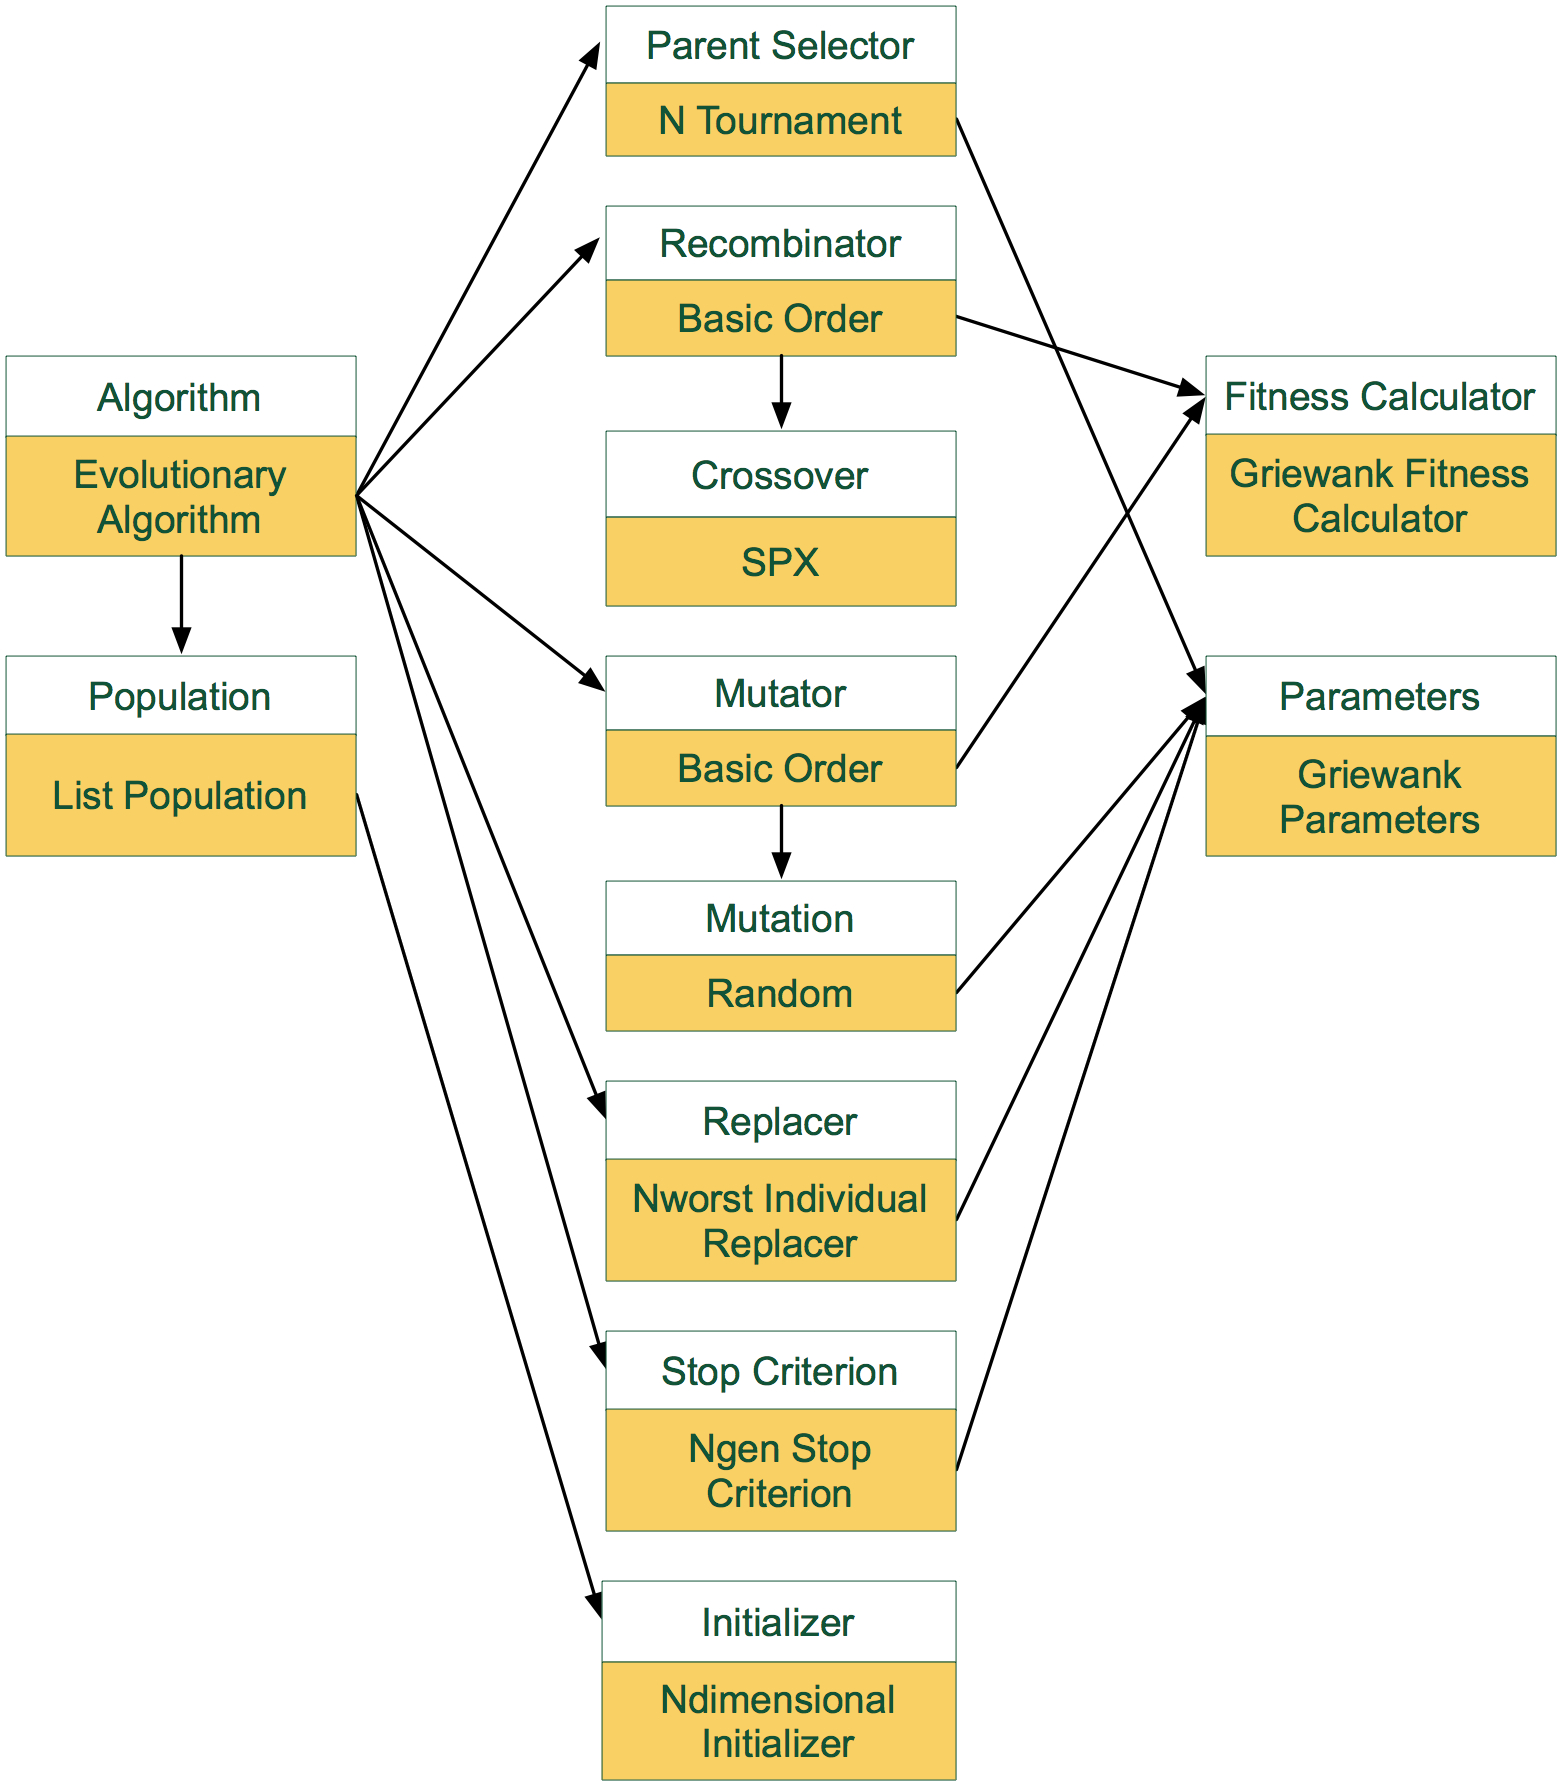
\includegraphics[width=10cm]{gfx/soaea/basicga.jpg}
\caption{Basic genetic algorithm. White blocks are interfaces and orange blocks are implementations. In this case, we are using specific implementations to solve the Griewank function problem.}
\label{BASICGAEXAMPLE}
\end{SCfigure}





Figure \ref{BASICGAEXAMPLE} shows a complete service oriented genetic algorithm, taking into account the proposed ideas. In this figure (and in the following ones) white blocks are the service interfaces. Orange blocks are specific implementations of these interfaces (that is, the source-code of the service), and  arrows indicate how a service implementation can make use of other services via their interface. For example, almost all implementations access to the {\em Parameters} service using its interface. Service implementations (orange blocks) can be selected in a configuration file or be automatically bound when they are available (among other options).



 The change from a problem instance to another is quite simple. It is only necessary to notify the algorithm a change in the implementation of the service {\em Fitness Calculator} and the implementation of {\em Parameters} (because these can vary from a problem to another). Because some algorithms need to calculate the fitness every time an individual is modified (and not only at the end of a generation) the Figure \ref{BASICGAEXAMPLE} shows how the service {\em Fitness Calculator} may be used inside the implementations that modify individuals ({\em Initializer}, {\em Mutator} or {\em Recombinator}). Moreover, each service can be in the local machine or distributed on the Internet, having the same behaviour.

%\subsection{Implementing a service oriented NSGA-II}
%\label{sec:nsga2}

As this is a iterative and incremental approach, other services can be discovered and designed in this step. For example, the difference between the previous version of a GA and the well known NSGA-II \cite{NSGA2} lies in the selection operator. Therefore, to change from the basic GA to NSGA-II, the mutator and crossover are kept and new selection operators are added. Figure \ref{fig:nsga2} shows the service oriented version of NSGA-II algorithm, where the new implementations are marked with a thick border. The problem has also been set to the multi-objective function MOP2 \cite{ReviewMultiobj06}. New auxiliary services have been added, like {\em Crowding Distance Assignator} or {\em Pareto Assignator}. As these services may be used in other algorithms in the future, they should be designed as abstract as possible. These new services are called from the implementation (code) of the services {\em NSGA-II Replacer} or {\em Binary Crowding Distance Selector} (black arrows indicate an interface call). 




\begin{SCfigure}[20][htb]
\centering
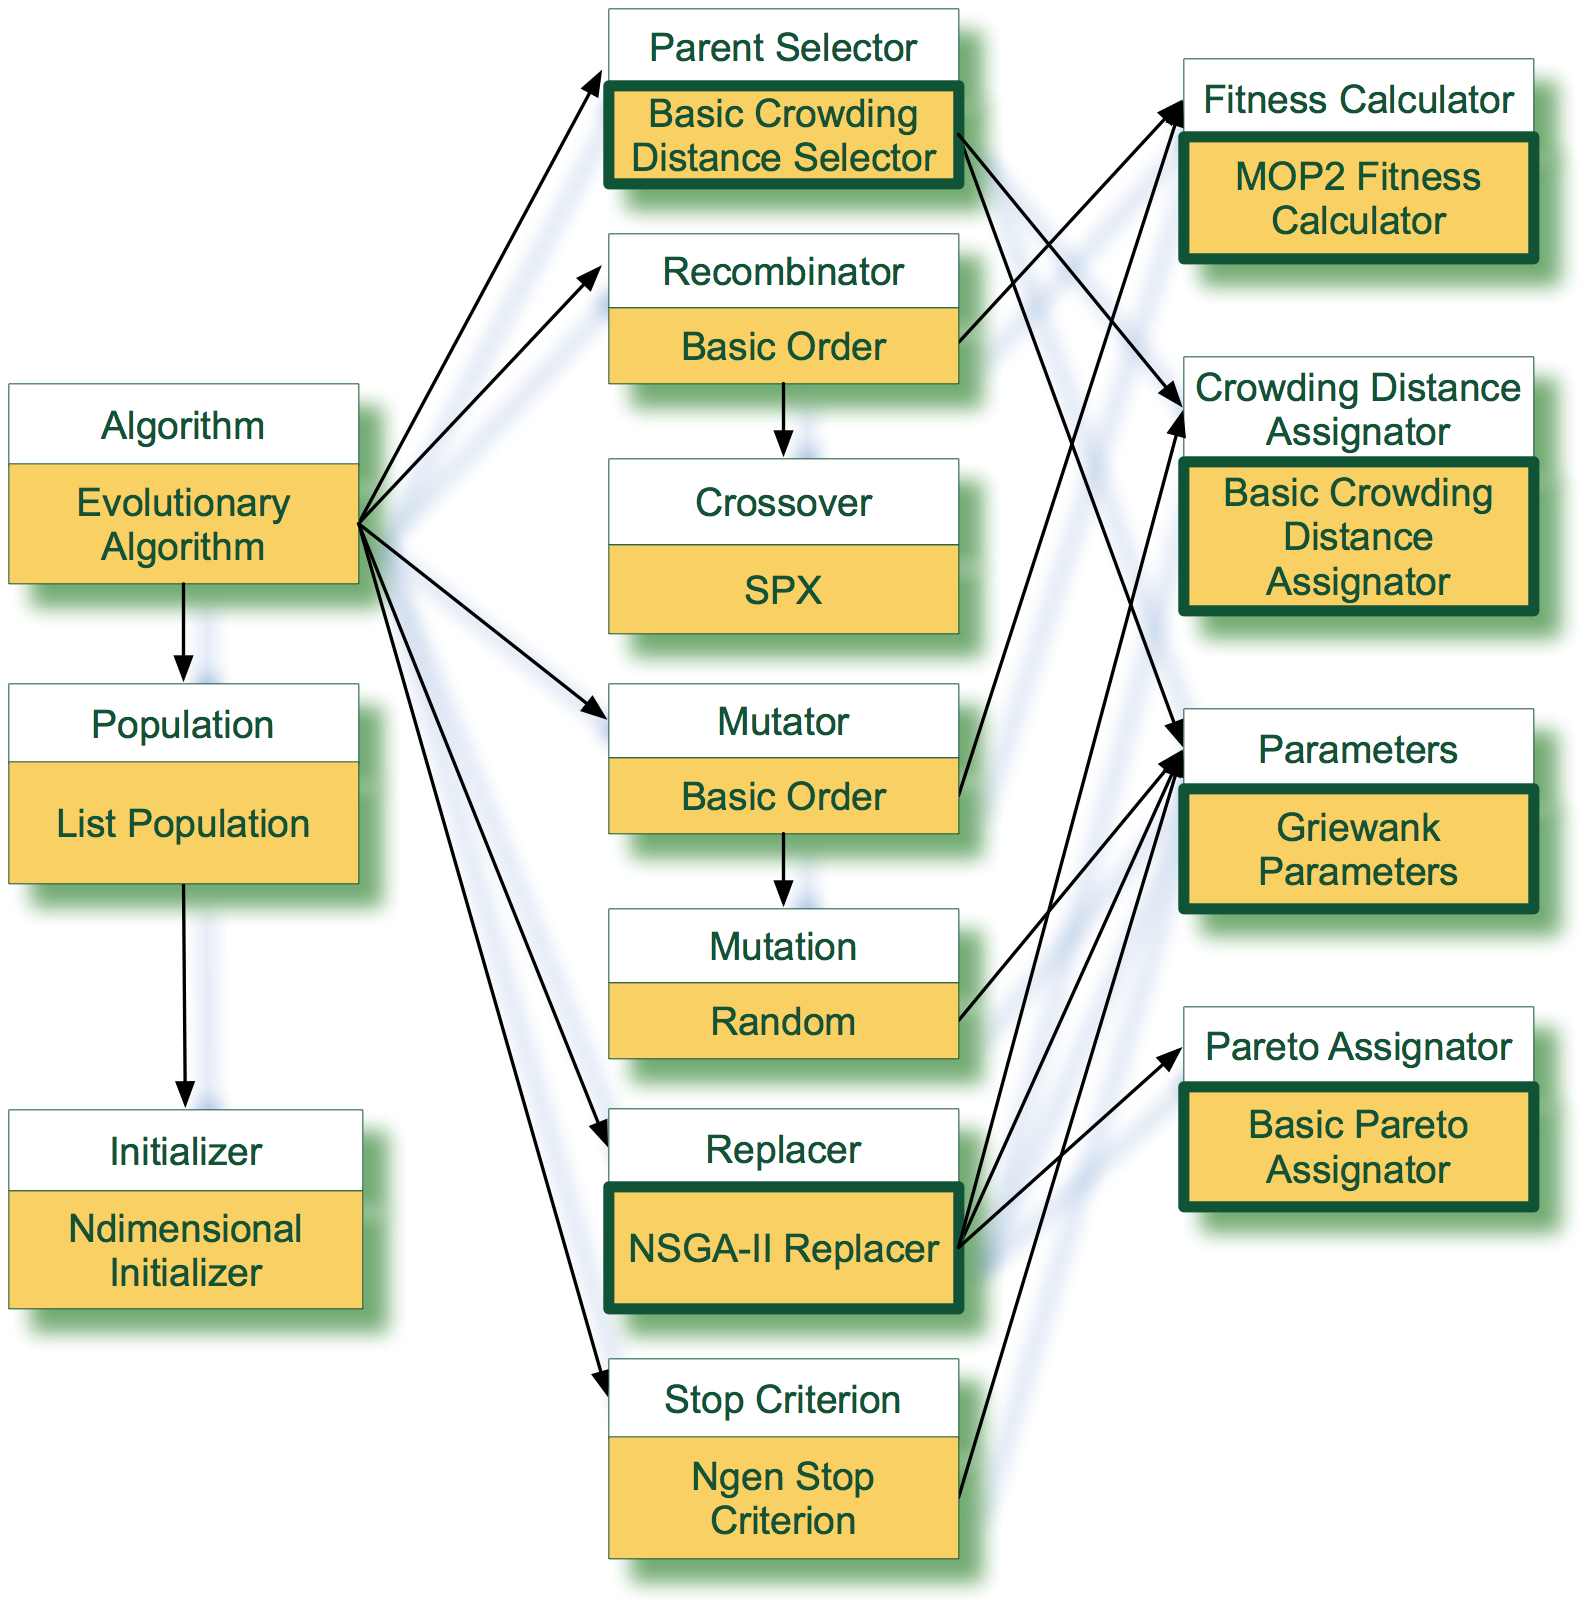
\includegraphics[width=10cm]{gfx/soaea/nsga2.jpg}
\caption{Modification of the basic GA adding new service implementations (orange blocks with thick lines).}
\label{fig:nsga2}
\end{SCfigure}



\subsection{Adding basic distribution}
\label{sec:distribution}

As every service must keep the same behaviour, independently of the machine that hosts it, distribution services for load balancing of a specific service can be easily created, for example, notifying the algorithm to use a distributed implementation for that service. As previously stated, the service {\em Fitness Calculator} receives a list of individuals to calculate their fitness, so, in this example, the new fitness implementation ({\em Basic Fitness Distributor}) binds with every fitness service available (in the same machine or in a network). The source code of this basic implementation simply distributes the list of individuals among the bound services and waits for their termination. Although more complex implementations probably will be more efficient, the objective of this section is to show how to distribute services, thus, this basic implementation is sufficient. Figure \ref{FITNESSDISTRIBUTOR} shows the modification from a sequential fitness calculator to a distributed one. Thanks to SOA, the number of distributed fitness calculators is not fixed: calculators can be added o removed in real time without stopping the system. As can be see in the figure, if one of the nodes is a cluster, it could also  implement another fitness distributor. This easy example can be adapted to more complex necessities depending on the infrastructure or the problem to be solved. More complex distribution services can be created, for example, taking into account communication latencies or computation capabilities of the nodes.




\begin{SCfigure}[20][htb]
\centering
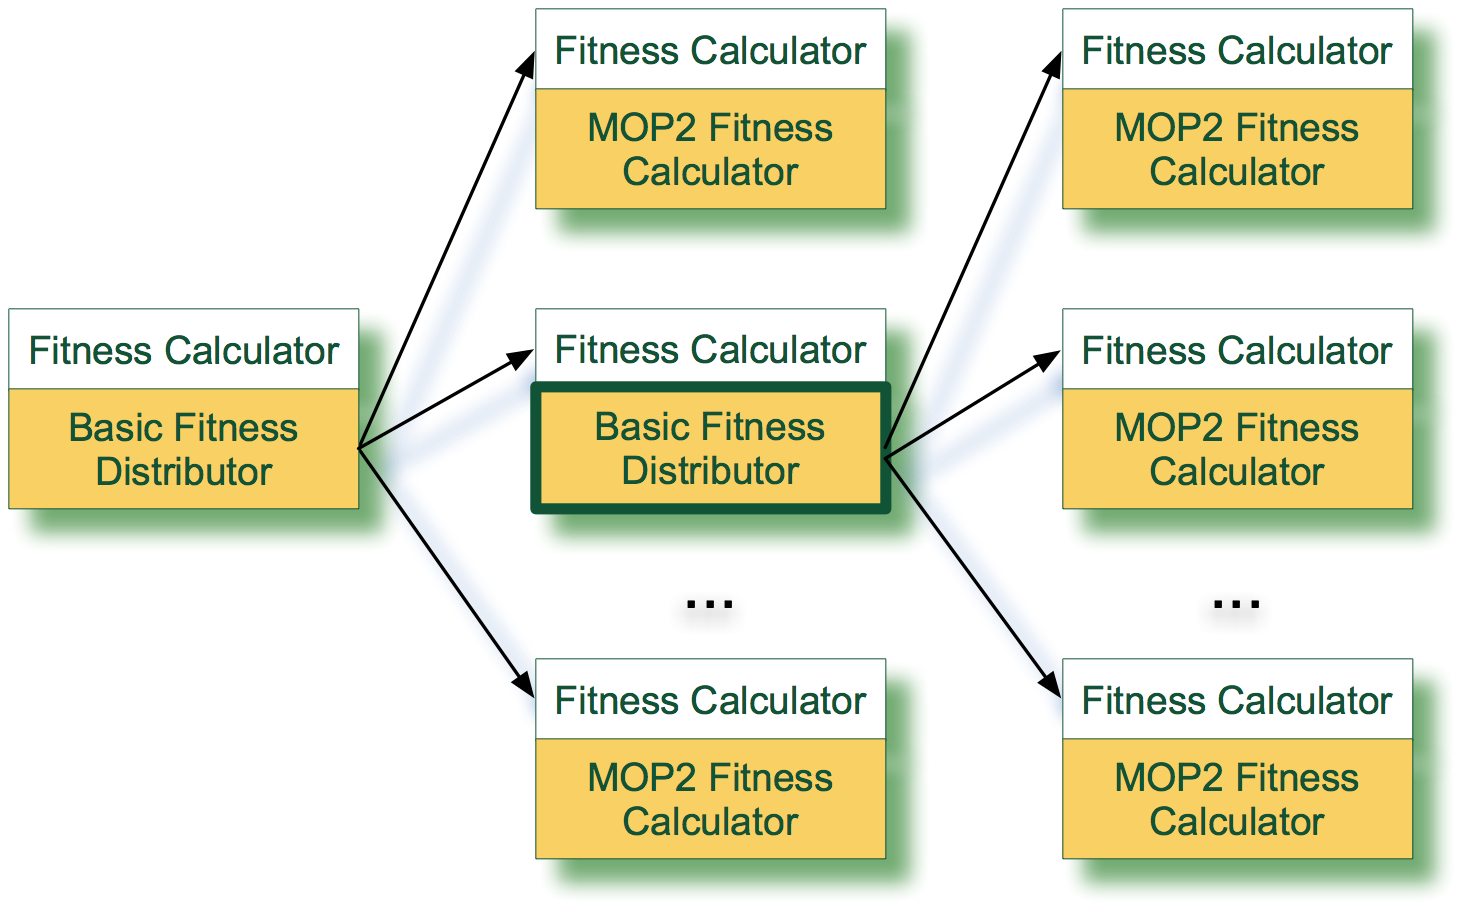
\includegraphics[width=10cm]{gfx/soaea/distributor.jpg}
\caption{Fitness distributor. The thick line implementation also re-distribute the individuals.}
\label{FITNESSDISTRIBUTOR}
\end{SCfigure}



One of the most extended model in parallel EAs is the island model. Using SOA-EA, the {\em Population} service implementation can be modified to become a distributed population. Each certain time, this population could exchange individuals with other populations modified by other algorithms. These populations should be added or deleted in execution time without affecting the algorithm execution. Figure \ref{POPULATION} shows this example, where a {\em Replacer} implementation maintains a list of references to other {\em Population} interfaces (which can be local or remote). Also other {\em Population} implementations exist ({\em List Population} is the usual list of individuals). If one of these population services drop, the others can continue working. The topology of these islands can also be managed from services (such as {\em Basic Replacer} service, or another). The  modification and dynamism of the population structure is difficult to apply in existing frameworks without using SOA because it is necessary to create mechanisms to modify the population behaviour, the operators to modify it, the data structures, and also the code to manage all. With he usage of SOA, and due to the capability of accessing to a population via its service interface, it is not necessary to modify the source code to modify the population and its behaviour. Also, to avoid bottlenecks in distributed executions, asynchronous communication must be provided to avoid idle time. This kind of communication offers excellent performance when working with different nodes and operating systems, as demonstrated by \cite{Alba2002Heterogeneous}.



\begin{SCfigure}[20][htb]
\centering
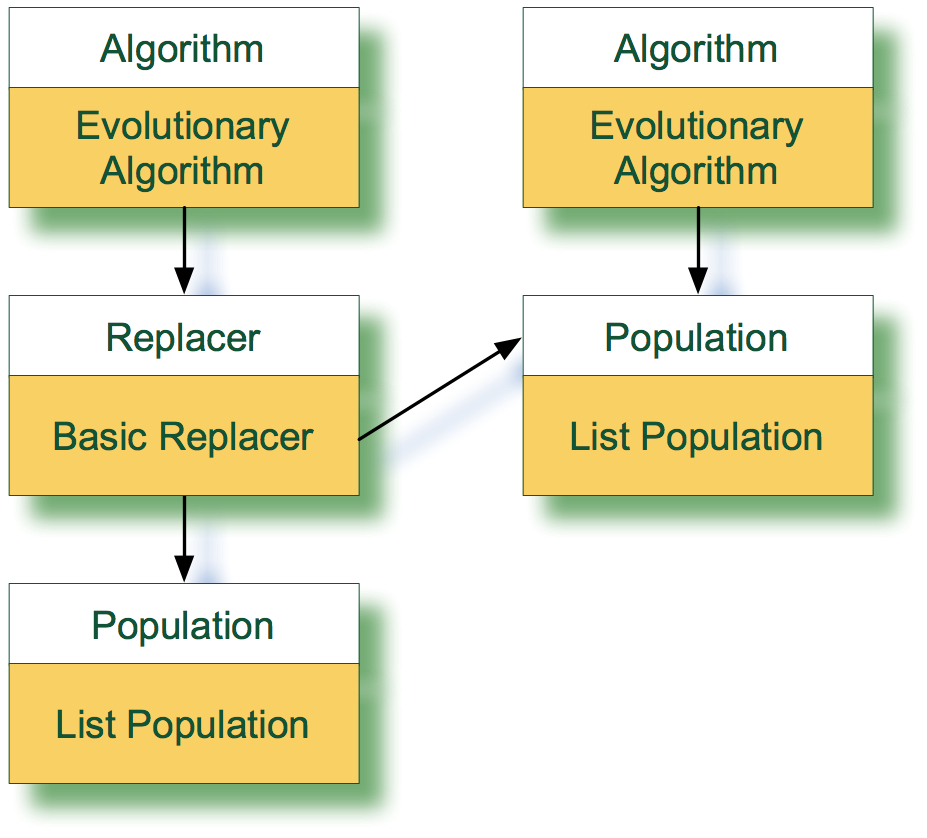
\includegraphics[width=7cm]{gfx/soaea/island.jpg}
\caption{Island model. From time to time, the Basic Replacer Implementation could send or receive individuals from other islands.}
\label{POPULATION}
\end{SCfigure}



\subsection{Self-adaptation in SOA-EA}
\label{sec:otherexamples}
There are several ways to create self-adaptable algorithms using SOA-EA. For example, creating a service that modifies the parameters in the {\em Parameters} service, or activating and de-activating operators in real time. An easier way is to create a service that manages all available services of the same kind. For example a {\em Mutator} service that binds all the available mutation implementations and use the most adequate one depending on some rules during the execution \cite{SelfadaptationSerpell2010}.  This idea can also be extended to create a service that implements several interfaces and selects the most adequate implementation for each interface respect to some criteria, as can be seen in Figure \ref{INTELLIGENTALGORITHM}, where thick lines represent the implementations used at the current moment (they vary as time passes).



\begin{SCfigure}[20][htb]
\centering
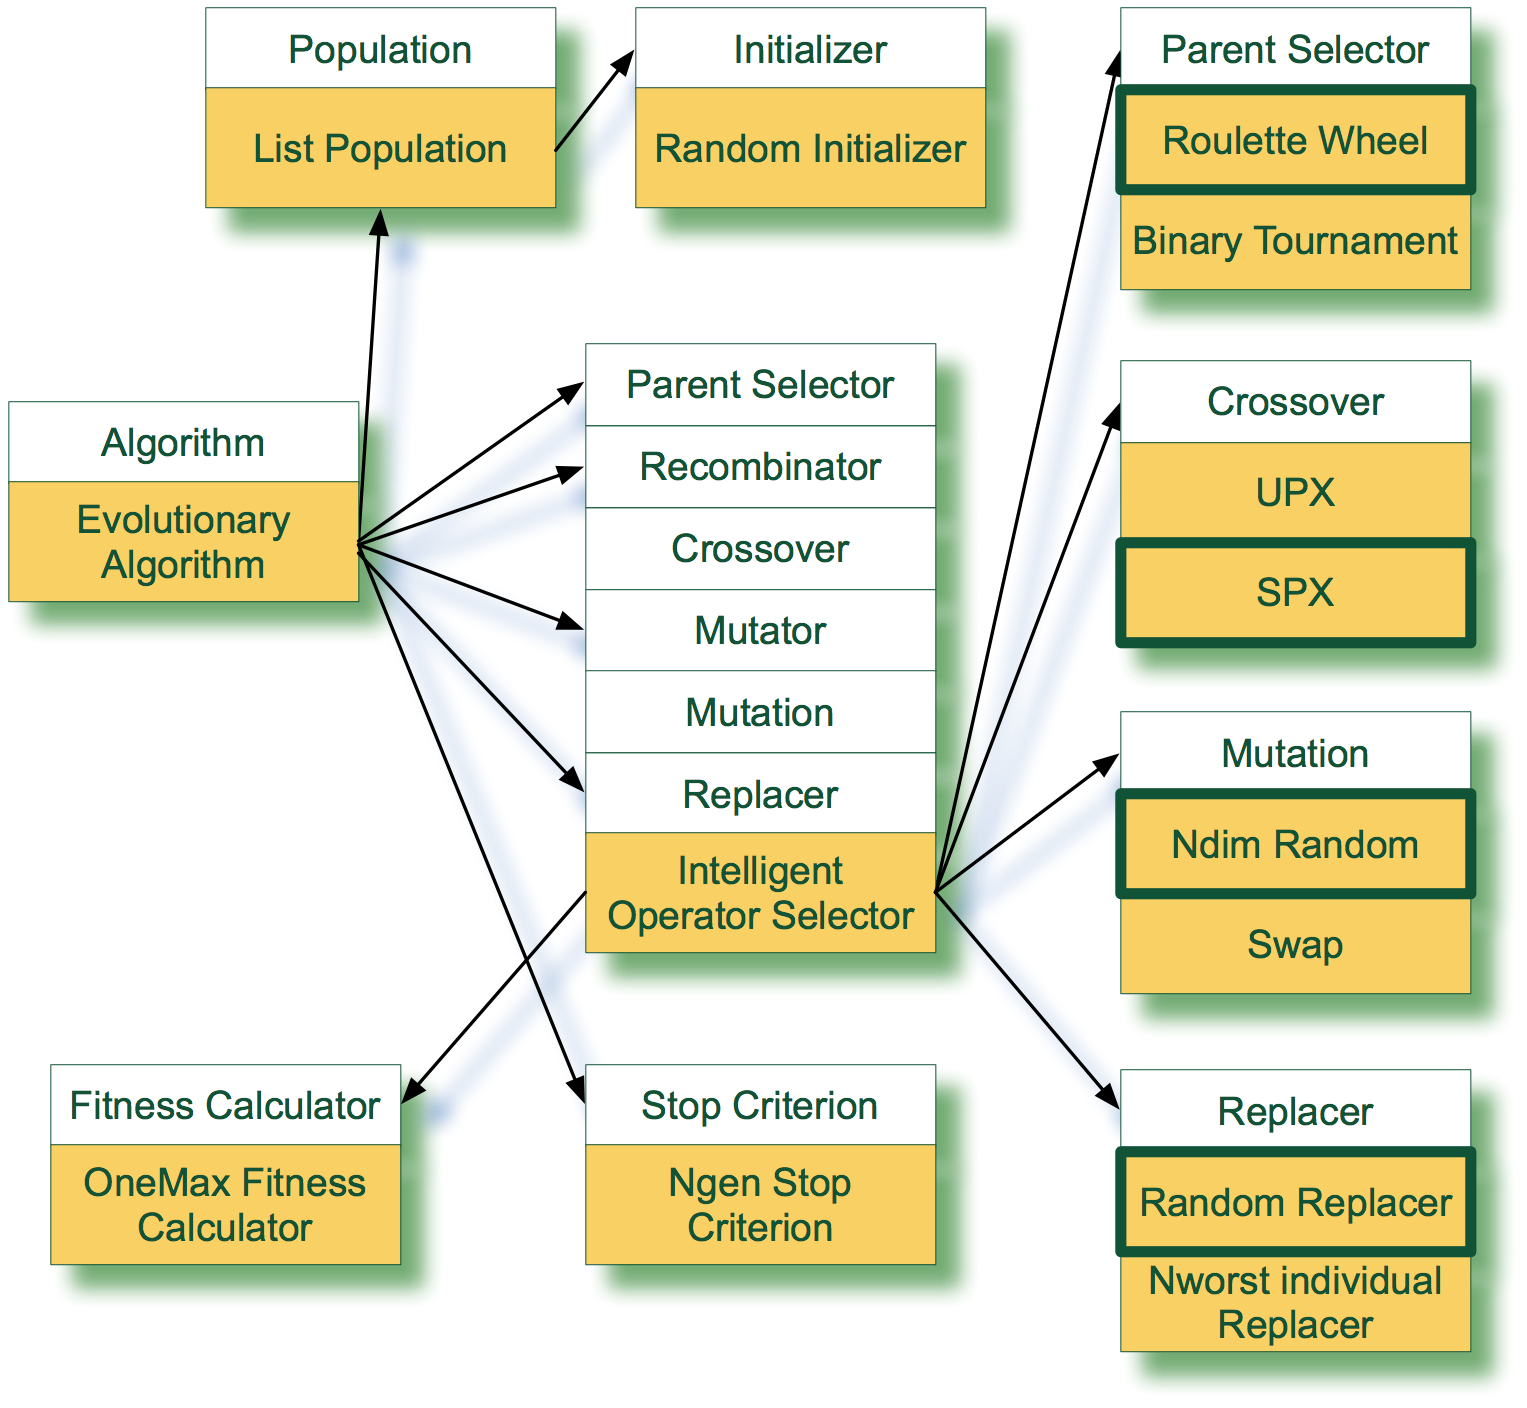
\includegraphics[width=10cm]{gfx/soaea/intelligent.jpg}
\caption{Self-adaptable Algorithm. The {\em Intelligent Operator Selector} selects which service implementation is used each time.}
\label{INTELLIGENTALGORITHM}
\end{SCfigure}


Finally, another important usage of EAs is its hybridization with other metaheuristics, to obtain more effective search algorithms \cite{HybridRodriguez2012},  increasing the performance of intensification and diversification mechanisms. With  traditional frameworks this task can be difficult, mainly because the source code for each metaheuristic must be modified. Nevertheless, using SOA a combination of loosely coupled services could be used.

\section{Conclusions}
%In this chapter we have presented the requirements in the EA design: generic representation, generic fitness, generic operations, generic evolutionary model, parameter management and configurable output. On the other hand, the requirements in SOA have been also shown: genericity in the service interfaces, programming language independence, distribution transparency and flexibility. 
In this chapter the requirements in EA design (genericity in representation, fitness, operations, model, parameters and output), with the requirements in SOA (genericity in interfaces, language independence, distribution and dynamism) have been taken into account to propose a methodology to model the services that compose a generic EA, and several guidelines about the design of these services have been explained. We have presented the steps to create a service-oriented evolutionary algorithm that takes advantages of the SOA capabilities. It has been explained how to modify the services to change from a model to another, adding transparent distribution and load-balancing or dynamic adaptation of the parameters.

Table \ref{tab:reasons} shows the advantages to design the elements of the EA as services.

\begin{SCtable}[][t]

\resizebox{11cm}{!}{
\begin{tabular}{p{2cm}p{2.5cm}p{3cm}p{7cm}}
%\begin{tabular}{llll}
%\noalign{\smallskip}\hline\noalign{\smallskip}
\hline
\rowcolor{colorCorporativoSuave}\textbf{Element} & \textbf{Current EAs development} & \textbf{Using SOA} & \textbf{Reason to migrate} \\
\hline \hline
%\rowcolor{colorCorporativoMasSuave}\noalign{\smallskip}\hline\noalign{\smallskip}
\rowcolor{colorCorporativoMasSuave}{\em Programming language} & Just one for all elements of the algorithm & Any & Services are independent of the programming language. Only the interface is required to use services  \\\hline
\rowcolor{colorCorporativoSuave}{\em Operators} & Methods or functions & Services & Services allow the selection of a specific implementation during the algorithm execution, and also different programming languages or distribution models\\\hline
\rowcolor{colorCorporativoMasSuave}{\em Operators behaviour} & Methods applied to a single individual & Service that receive individual lists  & It allows  load balancing and distribution, and also to modify the operators in execution time\\\hline
\rowcolor{colorCorporativoSuave}{\em Operator selection} & Modifying the source code & In a flexible way outside the source code & It is not mandatory to recompile the source code to integrate new operators \\\hline
\rowcolor{colorCorporativoMasSuave}{\em Fitness} & Method that evaluates an individual & Service that evaluates an individual list & It allows the distribution, load balancing and addition of new fitness calculators in real time \\\hline
\rowcolor{colorCorporativoSuave}{\em Population} & Array or individual list & Population service & It allows to change the population type and topography, by selecting the service implementation \\\hline
\rowcolor{colorCorporativoMasSuave}{\em Self-adaptation} & Modifying source code for a specific experiment & Self-adapting service that selects specific operator implementations & It does not modify the created services and brings more flexibility in the dynamic adaptation \\\hline
\rowcolor{colorCorporativoSuave}{\em Distribution} & Libraries like MPI & SOA mechanisms & SOA technologies allow changing the transmission protocol and using extra technologies without adding extra code\\
%\noalign{\smallskip}\hline
\hline
\end{tabular}
}
\caption{Summary of migration from traditional EA programming to SOA}

\label{tab:reasons}
\end{SCtable}

In next chapter, we will use a specific SOA technology (OSGi) to implement all the examples shown in previous sections, and how to accomplish the requirements in the development of EAs and SOA, taking advantage of the capabilities of SOA.


